\documentclass[12pt,english,brazil,a4paper,utf8,oneside]{utfpr-tcc}
% insere a margem no primeiro paragrafo
\usepackage{indentfirst}
% carrega o arquivo configuracoes.tex que contém os pacotes e comandos Latex.
%
% Esse arquivo conterá pacotes e comandos utilizados na monografia
%
% Observação - devido a um erro do sharelatex foi necessário colocar na raiz do projeto os seguintes arquivos:
% gcnumparser.sty, fcprefix.sty, fmtcount.sty, fc-poruges.def, fcportuguese.def.
% Tal problema foi relatado em: https://github.com/nlct/fmtcount/issues/26
% Quando o sharelatex corrigir o problema acredito que podemos remover esses arquivos do projeto. At. Luiz Arthur.
%

% Este comando não é necessário: utilizei apenas para deixar o latex2rtf
% feliz (e descobrir a codificação do texto).
\usepackage[utf8]{inputenc}

% Suporte a figuras e subfiguras
\usepackage{graphics}
\usepackage{subfigure}

% Suporte a tabelas (principalmente do cronograma)
\usepackage{tabularx}
\usepackage{multirow}
\usepackage{array}
\usepackage{tabularx}
\usepackage{colortbl}
\usepackage{hhline}
\usepackage{xcolor}

% Escalar fontes para redimencionar, por exemplo tabelas
\usepackage{scalefnt}

% Algoritmos.
\usepackage{algorithm,algorithmic}

\usepackage[alf]{abntex2cite}

% Elementos geralmente utilizados na tabela do cronograma
\newcommand{\fullcell}{\multicolumn{1}{>{\columncolor[gray]{0.5}}c}{}}
\newcommand{\fullcellline}{\multicolumn{1}{>{\columncolor[gray]{0.5}}c|}{}}
\newcommand{\mc}[3]{\multicolumn{#1}{#2}{#3}}
\newcommand{\y}{\rule{8pt}{4pt}}
\newcommand{\n}{\hspace*{8pt}}

% Define o caminho das figuras
\graphicspath{{images/}}

%% Configuração de glossário
\usepackage[portuguese]{nomencl}
\usepackage[nogroupskip,acronym,nomain,nonumberlist,nopostdot,nohypertypes={acronym}]{glossaries}

\makenoidxglossaries

% para siglas em português
\newcommand{\sigla}[2]
{
 \newglossaryentry{#1}{
  name=#1,
  description={#2},
  first={#2 (#1)},
  long={#2}
 }  
}

% para siglas de língua estrangeira, nessas a descrição longa fica em itálico.
\newcommand{\siglaIt}[2]
{
 \newglossaryentry{#1}{
  name=#1,
  description={\textit{#2}},
  first={#2 (\textit{#1})},
  long={\textit{#2}}
 }  
}

% --- Estilos para apresentação de Código ----- %
\usepackage{listings}
\lstloadaspects{formats}

% Opções de listing usados para o código fonte
% Ref: http://en.wikibooks.org/wiki/LaTeX/Packages/Listings

\lstset{ %
language=Java,                  % choose the language of the code
basicstyle=\footnotesize,       % the size of the fonts that are used for the code
%basicstyle=\ttfamily,
stringstyle=\ttfamily\color[rgb]{0.16,0.16,0.16},
numbers=left,                   % where to put the line-numbers
numberstyle=\footnotesize,      % the size of the fonts that are used for the line-numbers
stepnumber=1,                   % the step between two line-numbers. If it's 1 each line will be numbered
numbersep=4pt,                  % how far the line-numbers are from the code
showspaces=false,               % show spaces adding particular underscores
showstringspaces=false,         % underline spaces within strings
showtabs=false,                 % show tabs within strings adding particular underscores
frame=single,	                % adds a frame around the code
framerule=0.6pt,
tabsize=2,	                % sets default tabsize to 2 spaces
captionpos=b,                   % sets the caption-position to bottom
breaklines=true,                % sets automatic line breaking
breakatwhitespace=false,        % sets if automatic breaks should only happen at whitespace
escapeinside={\%*}{*)},         % if you want to add a comment within your code
backgroundcolor=\color[rgb]{1.0,1.0,1.0}, % choose the background color.
rulecolor=\color[rgb]{0.8,0.8,0.8},
extendedchars=true,
xleftmargin=10pt,
xrightmargin=10pt,
framexleftmargin=10pt,
framexrightmargin=10pt
}

\definecolor{javared}{rgb}{0.6,0,0} % for strings
\definecolor{javagreen}{rgb}{0.25,0.5,0.35} % comments
\definecolor{javapurple}{rgb}{0.5,0,0.35} % keywords
\definecolor{javadocblue}{rgb}{0.25,0.35,0.75} % javadoc

\definecolor{DarkBlue}{rgb}{0,0,0.61}
\definecolor{DarkGreen}{rgb}{0,0.4,0}

% Numeros.
\lstdefinestyle{mynumbers}{
	numbers=left,
	stepnumber=1,
	numbersep=4pt,
	numberstyle=\tiny\color{black}
}
% Text Code.
\lstdefinestyle{mytextcode}{
	basicstyle=\footnotesize,
	tabsize=2,
	showspaces=false,
	showstringspaces=false,
	extendedchars=true,
	breaklines=true
}
% Frame.
\lstdefinestyle{myframe}{
	backgroundcolor=\color{white},
	frame=trbl
}
% C++ Style.
\lstdefinestyle{C++}{
	language=C++,
	style=mynumbers,
	style=mytextcode,
	style=myframe,
  keywordstyle=\color{black}\bfseries,
  stringstyle=\color{gray},
  commentstyle=\color[rgb]{0.08,0.08,0.08},
  morecomment=[s][\color{lightgray}]{/*}{*/},
  otherkeywords={\#include, \#define, \#pragma, \#typedef, dim3},
  emph={ __device__, __global__, __shared__, __host__, __constant__},
  emphstyle=\color{DarkBlue}\bfseries,
  emph={[2] printf, scanf},
  emphstyle=[2]\color{DarkGreen},
}
% C Style.
\lstdefinestyle{C}{
	language=C,
	style=mynumbers,
	style=mytextcode,
	style=myframe,
	keywordstyle=\color{black}\bfseries,
  	stringstyle=\color{gray},
  	commentstyle=\color[rgb]{0.08,0.08,0.08},
  	morecomment=[s][\color{lightgray}]{/*}{*/},
  	otherkeywords={\#include, \#define, \#pragma, \#typedef, dim3, bool},
  	emph={ __device__, __global__, __shared__, __host__, __constant__},
  	emphstyle=\color{DarkBlue}\bfseries,
  	emph={[2] printf, scanf},
  	emphstyle=[2]\color{DarkGreen},
	backgroundcolor={}
}
% Bash Style.
\lstdefinestyle{bash}{
	language=bash,
	style=mynumbers,
	style=mytextcode,
	style=myframe,
	backgroundcolor={},
	frame=single,
	basicstyle=\scriptsize\ttfamily
}
% Python Style.
\lstdefinestyle{python}{
	language=python,
	style=mynumbers,
	style=mytextcode,
	style=myframe,
	backgroundcolor={}
}
% Java Style.
\lstdefinestyle{java}{
	language=java,
	style=mynumbers,
	style=mytextcode,
	style=myframe,
	backgroundcolor={}
}
% ASM Style.
\lstdefinestyle{asm}{
  %belowcaptionskip=1\baselineskip,
  %xleftmargin=\parindent,
  language=[x86masm]Assembler,
  style=mynumbers,
  style=mytextcode,
  style=myframe,
  backgroundcolor={},
  frame=single,
  basicstyle=\scriptsize\ttfamily,
  commentstyle=\itshape\color{purple!40!black},
}

% Fortran Style.
\lstdefinestyle{fortran}{
  language=[90]Fortran,
  style=mynumbers,
  style=mytextcode,
  style=myframe,
  backgroundcolor={},
  frame=single,
  basicstyle=\footnotesize,
  commentstyle=\itshape\color{purple!40!black},
  morecomment=[l]{!\ }% Comment only with space after !
}

% LLVM Style.
\lstdefinestyle{llvm}{
	language=llvm,
	%inputencoding=utf8,
	style=mynumbers,
	style=mytextcode,
	style=myframe,
	backgroundcolor={},
	frame=single,
	basicstyle=\scriptsize\ttfamily,
  tabsize=4,
  %rulecolor=,
  upquote=true,
% aboveskip={1.5\baselineskip},
  columns=fixed,
  prebreak = \raisebox{0ex}[0ex][0ex]{\ensuremath{\hookleftarrow}},
  showtabs=false,
	%basicstyle=\scriptsize\upshape\ttfamily,
  identifierstyle=\ttfamily,
  keywordstyle=\ttfamily\bfseries\color[rgb]{0,0,0},
  %commentstyle=\ttfamily\color[rgb]{0.133,0.545,0.133},
  commentstyle=\ttfamily\color[rgb]{0.08,0.08,0.08},
  %stringstyle=\ttfamily\color[rgb]{0.627,0.126,0.941}
  stringstyle=\ttfamily\color[rgb]{0.16,0.16,0.16}
}

\lstdefineformat{C}{%
	\{=\newline\string\newline\indent,%
	\}=[;]\newline\noindent\string\newline,%
	\};=\newline\noindent\string\newline,%
	;=[\ ]\string\space}

% --- Fim da Definição de Estilos para apresentação de Código ----- %
% carrega o arquivo constantes.tex que contém dados do curso/monografia que NÃO DEVEM ser alterados. 
% Dados do curso que não precisam de alteração
\university{Universidade Tecnológica Federal do Paraná}
\universityen{Federal University of Technology -- Paraná}
\universityunit{Departamento Acadêmico de Computação}
\address{Campo Mourão}
\addressen{Campo Mourão, PR, Brazil}
\documenttype{Monografia}
\documenttypeen{Monograph}
\degreetype{Graduação}
% carrega o arquivo variaveis.tex que contém dados do acadêmico/monografia que DEVEM ser alterados.
% Dados do curso. Caso seja BCC:
\program{Curso de Bacharelado em Ciência da Computação}
\programen{Undergradute Program in Computer Science}
\degree{Bacharel}
\degreearea{Ciência da Computação}
% Caso seja TSI:
% \program{Curso Superior de Tecnologia em Sistemas para Internet}
% \programen{Undergradute Program in Tecnology for Internet Systems}
% \degree{Tecnólogo}
% \degreearea{Tecnologia em Sistemas para Internet}


% Dados da disciplina. Escolha uma das opções e a descomente:
% TCC1:
\goal{Proposta de Trabalho de Conclusão de Curso de Graduação}
\course{Trabalho de Conclusão de Curso 1}
% TCC2:
% \goal{Trabalho de Conclusão de Curso de graduação}
% \course{Trabalho de Conclusão de Curso 2}


% Dados do TCC (precisa alterar)
\author{Ana Carolina Frozza}  % Seu nome
\title{Reconhecimento de acordes com vetores croma e metodo de classificação} % Título do trabalho
\titleen{} % Título traduzido para inglês
\advisor{Prof. Dr. Diego Bertolini} % Nome do orientador. Lembre-se de prefixar com "Prof. Dr.", "Profª. Drª.", "Prof. Me." ou "Profª. Me."}
% \coadvisor{} % Nome do coorientador, caso exista. Caso não exista, comente a linha.
\depositshortdate{2017} % Ano em que depositou este documento

% Dados da ficha catalografica. Ela é opcional, mas é uma boa ideia inserí-la. Exemplos para geração (http://fichacatalografica.sibi.ufrj.br/)
\fichacatautor{Frozza, Ana}  % Nome conforme citado (ou seja, no formato "Sobrenome, Nome").
\fichacatbib{Biblioteca da UTFPR de Campo Mourão} % Não alterar
\fichacatpum{M488} % Código Cutter-Sanborn. Use a primeira letra do sobrenome seguido do número conforme as primeiras letras do sobrenome e a tabela http://www.amormino.com.br/cutter-sanborn/cutter1.html
\fichacatpalcha{} % Assuntos do trabalho. Cada item deve ser enumerado e separado por ponto: 1. xxx. 2. yyy. 3. zzz.
\fichacatpdois{} % Deixar em branco

% carrega o arquivo listaabreviaturas.tex que está dentro do diretório pretextual, esse arquivo contém as siglas utilizadas na monografia.
% quando a sigla for de língua portuguesa utilize \sigla{SIGLA}{Significado em português}
% quando a sigla for de língua estrangeira utilize \siglaIt{SIGLA}{Significado em Inglês}

\sigla{UTFPR}{Universidade Tecnológica Federal do Paraná}
% \siglaIt{ACM}{\textiAssociation for Computing Machinery}
\siglaIt{IP}{Internet Protocol}
\siglaIt{MIDI}{Musical Instruments Digital Interface}
\siglaIt{PCP}{Pitch Class Profiles }
\siglaIt{FFT}{Fast Fourier Transform}

% No texto quando for utilizar a sigla utilize os seguintes comandos:
%\acrlong{label} - acronimo/sigla longo
%\acrshort{label} - acronimo/sigla curta
%\Gls{TCP} - sigla com o significado primeiro em Maiusculo
%\GLS{TCP} - sigla com o significado tudo em MAIUSCULO
%\gls{TCP} - sigla com o significado tudo em minusculo % usando glossaries

\begin{document}
	
\frontmatter
\maketitle

% carrega o arquivo resumo.tex que está dentro do diretório pretextual, esse arquivo deve conter o resumo da monografia.
\begin{resumo}
%Elemento obrigatório, constituído de uma sequência de frases concisas e objetivas, em forma de texto.  Deve apresentar os objetivos, métodos empregados, resultados e conclusões.  O resumo deve ser redigido em parágrafo único, conter no máximo 500 palavras e ser seguido dos termos representativos do conteúdo do trabalho (palavras-chave).


TEXTO TEXTO TEXTO TEXTO TEXTO TEXTO TEXTO TEXTO TEXTO TEXTO TEXTO TEXTO TEXTO TEXTO TEXTO TEXTO TEXTO TEXTO TEXTO TEXTO TEXTO TEXTO TEXTO TEXTO TEXTO TEXTO TEXTO TEXTO TEXTO TEXTO TEXTO TEXTO TEXTO TEXTO TEXTO TEXTO TEXTO TEXTO TEXTO TEXTO TEXTO TEXTO TEXTO TEXTO TEXTO TEXTO TEXTO TEXTO TEXTO TEXTO TEXTO TEXTO TEXTO TEXTO TEXTO TEXTO TEXTO TEXTO TEXTO TEXTO TEXTO TEXTO TEXTO TEXTO TEXTO TEXTO TEXTO TEXTO TEXTO TEXTO TEXTO TEXTO TEXTO TEXTO TEXTO TEXTO TEXTO TEXTO TEXTO TEXTO TEXTO TEXTO TEXTO TEXTO TEXTO TEXTO TEXTO TEXTO TEXTO TEXTO TEXTO TEXTO TEXTO TEXTO TEXTO TEXTO TEXTO TEXTO TEXTO TEXTO TEXTO TEXTO TEXTO TEXTO TEXTO TEXTO TEXTO TEXTO TEXTO TEXTO TEXTO TEXTO TEXTO TEXTO TEXTO TEXTO TEXTO TEXTO TEXTO TEXTO TEXTO TEXTO TEXTO TEXTO TEXTO TEXTO TEXTO TEXTO TEXTO TEXTO TEXTO TEXTO

% TODO: se possível, escreva um resumo estruturado. Para TCC 1, o resumo estruturado teria os seguintes elementos:
% \textbf{Contexto:} \\
% \textbf{Objetivo:} \\
% \textbf{Método:} \\
% \textbf{Resultados esperados:} 
% ou, para TCC 2:
% \textbf{Contexto:} \\
% \textbf{Objetivo:} \\
% \textbf{Método:} \\
% \textbf{Resultados:} \\
% \textbf{Conclusões:}

% Palavras-chaves, separadas por ponto (tente não definir mais do que cinco)
\palavraschaves{}
\end{resumo}
% carrega o arquivo abstract.tex que está dentro do diretório pretextual, esse arquivo deve conter um resumo escrito na linguá inglesa para a monografia.
%% Caso seja TCC 2, precisa traduzir o resumo e as palavras-chaves para inglês:
\begin{abstract}
Put the abstract here...

TEXT TEXT TEXT TEXT TEXT TEXT TEXT TEXT TEXT TEXT TEXT TEXT TEXT TEXT TEXT TEXTTEXT TEXT TEXT TEXT TEXT TEXT TEXT TEXTTEXT TEXT TEXT TEXT TEXT TEXT TEXT TEXTTEXT TEXT TEXT TEXT TEXT TEXT TEXT TEXTTEXT TEXT TEXT TEXT TEXT TEXT TEXT TEXTTEXT TEXT TEXT TEXT TEXT TEXT TEXT TEXTTEXT TEXT TEXT TEXT TEXT TEXT TEXT TEXTTEXT TEXT TEXT TEXT TEXT TEXT TEXT TEXTTEXT TEXT TEXT TEXT TEXT TEXT TEXT TEXTTEXT TEXT TEXT TEXT TEXT TEXT TEXT TEXTTEXT TEXT TEXT TEXT TEXT TEXT TEXT TEXTTEXT TEXT TEXT TEXT TEXT TEXT TEXT TEXTTEXT TEXT TEXT TEXT TEXT TEXT TEXT TEXTTEXT TEXT TEXT TEXT TEXT TEXT TEXT TEXTTEXT TEXT TEXT TEXT TEXT TEXT TEXT TEXT
% \textbf{Context:}
% \textbf{Objective:}
% \textbf{Method:}
% \textbf{Results:}
% \textbf{Conclusions:}

% Palavras-chaves em inglês, separadas por ponto.
% \keywords{}
\end{abstract}

% Listas (opcionais, mas recomenda-se a partir de 5 elementos)
%\listoffigures
%\listoftables
%\listofacronyms
\printnoidxglossaries

% Sumário
\tableofcontents

\mainmatter

% Capítulos da monografia:
\chapter{Introdução}
\label{cap:introducao}

% Coloque aqui o texto da introdução, contextualizando o seu trabalho...

% Testando o uso das siglas na \gls{UTFPR} - pela primeira vez para \gls{ACM}. Segunda vez para \gls{ACM}...

% A rede \gls{IP}...

% Sugestões de seções
% \section{Considerações preliminares}

A transcrição musical automática é algo que a muito tempo atrai o interesse de muitos músicos. Transcrever uma música está associado ao ato de escutar e escrever o conteúdo que se ouviu. A motivação deste trabalho está na necessidade da criação de um software de reconhecimento de acordes musicais para auxiliar no aprendizado de novos músicos. 

Atualmente existem diversos aplicativos que fazem a tradução para \gls{MIDI}. Entretanto, por se tratar de uma tarefa extremamente complexa, a qualidade obtida na transcrição ainda é bastante limitada. 
Para realizar a transcrição de uma música, vários aspectos devem ser avaliados pelo software, como: o tempo, que é a velocidade em que a música é tocada; os instrumentos utilizados; a altura, que é a frequência das notas; o volume e a duração de cada nota. 

Devido a esta e outras dificuldades, foi adotado a cifra como notação musical, pois considera apenas a altura das notas. A análise de tipos de instrumentos musicais diferentes e ritmos foram ignorados. Como fonte sonora foi escolhido o violão, por se tratar de um instrumento popular e que normalmente é usado em  estudos de outros artigos, dos quais poderá comparar resultados com outros autores.


\section{Objetivos}
\label{cap:introducao:sec:objetivos}

O estudo tem como objetivo desenvolver um software capaz de identificar acordes utilizando transformada rápida de Fourier (FFT), vetor croma para detecção de acordes, além de redes Neurais para classificação. Este software poderá ser utilizado futuramente para um Sistema de Reconhecimento de acordes musicais mais complexos que seja capaz de distinguir outros instrumentos. 


\section{Problema de Pesquisa}
\label{cap:introducao:sec:problema:pesquisa}

No decorrer deste trabalho três preocupações estavam presentes:
Evitar que irregularidades na estimativa da frequência de referencia ocasionasse notas espúrias.
Eliminar o atraso decorrente do fato das notas muitas vezes não possuírem, em seu estagio inicial, altura definida.
Impedir que uma sequencia de notas repedidas seja interpretado como uma única nota.


% \section{Contribuições}
% \label{cap:introducao:sec:contribuicoes}

% No que o seu trabalho ajuda? Há diferenças entre o seu trabalho e outros?

\section{Organização do Texto}
\label{cap:introducao:sec:organizacao:texto}


O capítulo~\ref{cap:conceitos} apresenta alguns conceitos e ferramentas necessários para o desenvolvimento do trabalho. Uma introdução breve sobre os conceitos da música e suas notas, frequência e acordes, a transformada discreta de Fourier e a transformada rápida de Fourier, são revistas. Apresenta-se uma breve explicação sobre vetores croma. Ao fim, é descrito o funcionamento geral sobre redes neurais. Os trabalhos utilizados como referências são abordados no capítulo~\ref{cap:trabalhos:relacionados} .

A metodologia é discutida no capítulo~\ref{cap:metodologia}, onde será mostrada a implementação do sistema detalhadamente. Nele a estrutura principal do projeto é apontada, e as decisões tomadas são explicitadas. E finalmente, no capítulo~\ref{cap:proposta} é apresentada a proposta do seguinte trabalho e o cronograma de atividades a ser seguido. 

% Finalmente, no Capítulo~\ref{cap:conclusoes} obtem-se as considerações finais e as conclusões obtidas no desenvolvimento deste trabalho. 

% No Capítulo~\ref{cap:introducao} blablabla, no capítulo seguinte tititi, etc... Nossa proposta é apresentada no Capítulo~\ref{cap:proposta}.... Finalmente, no Capítulo~\ref{cap:conclusoes} apresentamos as conclusões obtidas no desenvolvimento deste trabalho...

\chapter{Conceitos}
\label{cap:conceitos}

%---------------------------------------------------%
\section{Introdução á Música}
\label{cap:conceitos:intr:musica}

De acordo com \cite{roads1996computer}, o som pode ser expresso por uma soma de funções periódicas. Sendo assim,
ele pode ser decomposto em combinações de funções matemáticas primitivas,
chamadas de seno ou senóides.

O som é medido fisicamente por sua intensidade, frequência e timbre.
\begin{enumerate}
	\item{\textbf{Intensidade:} é definido como volume ou amplitude do som;}
	\item{\textbf{Altura:} é definida como uma senóide mais grave ou  mais aguda, quanto mais grave, menor a frequência e quanto mais aguda, maior a frequência;}
	\item{\textbf{Timbre:} é como as senóides se diferem;}
\end{enumerate}

O ouvido humano pode reconhecer frequências de 20Hz à 20KHz, sendo
capaz de distinguir cerca de 1400 frequências discreta. Sons fora desse intervalo
não são percebidos porque não possuem energia suficiente para vibrar o tı́mpano,
ou porque a frequência é tão alta que o tı́mpano não consegue perceber.

Na relação entre duas frequências x e y, sendo a primeira mais baixa que a
segunda, temos a razão y/x. Quando dois sons tem relação de frequência 2:1
este recebe o nome de oitava.

Dentro da faixa de audição humana podemos distinguir 10 oitavas: 20Hz a
40Hz, 40Hz a 80Hz, 80Hz a 160Hz, 160Hz a 320Hz, 320Hz a 640Hz, 640Hz a
1280Hz, 1280Hz a 2560Hz, 2560Hz a 5120Hz, 5120Hz a 10240, 10240 a 20480Hz.

Uma nota musical é um som cuja a frequência de vibração encontra-se dentro
do intervalo perceptı́vel ao ouvido humano e a música é a combinação, sob as
mais diversas formas, de uma sequência de notas em diferentes intervalos.

As notas musicais Dó, Ré, Mi, Fá, Sol, Lá e Si, se repetem em intervalos
formando oitavas. Uma nota em um intervalo possui o dobro do valor da sua
frequência no intervalo anterior. Dessa forma, a nota Lá pertencente à quarta
oitava tem frequência 440Hz, no próximo intervalo dobra a frequência e pertence
à quinta oitava passando a ter 880Hz \cite{kostka2000tonal}.

Os 12 intervalos que compõem a oitava são chamados de semitons. Portanto
existem 12 semitons iguais em uma oitava. Dois semitons juntos formam um
tom. Um semitom separa uma nota de um acidente musical ou de outra nota.

Os acidentes musicais, bemol (b), sustenido ($\sharp$), alteram o valor da nota em um semitom para baixo ou para cima, respectivamente.

Sendo assim os acidentes C$\sharp$, D$\sharp$, F$\sharp$, G$\sharp$ e A, possuem respectivamente, as mesmas frequências dos acidentes Db, Eb, Gb, Ab e Bb quando soam na mesma oitava.

É possível construir uma tabela com as 7 oitavas destinadas ao conceito musical. A \cref{tabela} abaixo mostra o valor da frequência para uma nota ou acidente musical a partir na nota central Lá.
As sete oitavas estão representadas pelas colunas e os intervalos pelas linhas.

\begin{table}[!htb]
	\centering	
	\caption{Frequências sonoras}
	\label{tabela}
	\begin{tabular}	{|c|c|c|c|c|c|c|c|c|c|c|c|}
	\hline
	\multicolumn{2}{|c|}{Notas}  & 1 & 2 & 3 & 4 & 5 & 6 & 7 & 8 & 9 & 10  \\ \hline
		01 & C         & 32,70 & 65,41  & 130,82 & 261,63 & 523,25 & 1046,50 & 2093,00 & 4186,00 & 8372,00 & 16744,00 \\ \hline
		02 & C$\sharp$ & 34,65 & 69,30  & 136,60 & 277,20 & 554,37 & 1108,73 & 2217,46 & 4434,92 & 8869,84 & 17739,68 \\ \hline
		03 & D         & 35,71 & 73,42  & 146,83 & 293,66 & 567,33 & 1174,66 & 2349,32 & 4698,64 &  9397,28 & 18794,56 \\ \hline
		04 & D$\sharp$ & 36,70 & 77,78  & 155,57 & 311,13 & 622,25 & 1544,51 & 2469,01 & 4938,02 & 9876,04 & 19752,08 \\ \hline
		05 & E         & 20,06 & 41,20 & 82,41  & 164,81 & 329,63 & 659,25 & 1318,51 & 2637,02 & 5274,04 & 10548,08 \\ \hline
		06 & F         & 21,83 & 43,65 & 87,31  & 174,61 & 349,23 & 689,45 & 1396,92 & 2793,83 & 5587,66 & 11175,32 \\ \hline
		07 & F$\sharp$ & 23,12 & 46,25 & 92,50  & 184,99 & 369,99 & 739,99 & 1479,98 & 2959,95 & 5991,90 & 11983,80 \\ \hline
		08 & G         & 24,49 & 48,99 & 97,99  & 195,99 & 391,99 & 783,99 & 1567,89 & 3135,96 & 6271,92 & 12543,84 \\ \hline
		09 & G$\sharp$ & 25,95 & 51,91 & 103,02 & 207,65 & 415,30 & 830,60 & 1661,22 & 3322,44 & 6644,88 & 13289,76 \\ \hline
		10 & A         & 27,50 & 55,00 & 110,00 & 220,00 & 440,00 & 880,00 & 1760,00 & 3520,00 & 7040,00 & 14080,00 \\ \hline
		11 & A$\sharp$ & 29,13 & 58,27 & 116,54 & 233,10 & 466,16 & 932,33 & 1864,65 & 3729,31 & 7458,62 & 14917,24 \\ \hline
		12 & B         & 30,87 & 61,74 & 123,48 & 246,94 & 493,88 & 986,76 & 1975,53 & 3951,10 & 7902,20 & 15804,40 \\ \hline
	\end{tabular}
\end{table}

% OBS: como colocar a tabela pro lado ou virada na pagina

\subsection{Frequências, notas e acordes no violão}
O braço do violão popular é dividido em trastes, formando espaços chamados de casas. Dentro dessas casas as notas são separadas, uma das outras, por um semitom. As seis cordas ficam sobre o braço  e são organizadas da mais fina para a mais grossa, ou da frequência mais alta para a mais baixa, olhando o violão de baixo para cima.

A afinação deste instrumento é dita “afinação em quartas”, pois depois de um intervalo de quarto casas a frequência passa a ser a mesma da corda imediatamente abaixo desta.

Três ou mais notas tocadas juntas formam um acorde. Os acordes são formados por intervalos harmônicos dando um sentido na harmonia. Os acordes menores e maiores são chamados de tríade, pois precisam apenas de três notas para a escala.

Acordes Maiores: Essa escala é construída respeitando a distribuição de Tons e Semitons (T-T-ST-T-T-T-ST). Ex: A partir da nota C seguindo a distribuição, temos, C, D, E, F, G, A, B e C.

Acordes Menores: É possível criar um acorde menor a partir da escala menor e respeitando a distribuição de Tons e Semitons (T-ST-T-T-ST-T-T). Ex: A partir de C seguindo a distribuição anterior, temos, C, D, Eb, F, G, Ab, Bb, C.

O acorde no violão é representado pelas notas que formam a repetição e de algumas destas devido a quantidade de cordas que vibram ao mesmo tempo ser maior que a necessárias para a formação dos acordes. Logo os acordes menores e maiores do violão são formados pela tríade e pela repetição de alguma destas notas.
 

%---------------------------------------------------%
\section{Transformada Rápida de Fourier}
\label{cap:conceitos:TTF}

%Escrever mais sobre a trasformada de fourier e qual a importancia dela para este trabalho

A Transformada rápida de Fourier (\gls{FFT}) é uma representação de uma função periódica de grande importância para processamento digital de sinais.

A FFT é um algoritmo eficiente para se calcular a Transformada discreta de Fourier e a sua inversa. 

O método de cálculo da transformada discreta de Fourier a partir da expressão
\begin{equation} \label{eq1}
\begin{split}
Fn & = f_k e^{-i2\pi n\frac{k}{N}} = \sum_{k=0}^{N-1} f_k W^{k n} ,n = 0,...,N-1 
\end{split}
\end{equation}
utiliza \(N^2\) produtos entre números complexos e \(N(N-1)\) somas, possuindo assim complexidade computacional \(O(N^2)\).
O método FFT permite obter o mesmo resultado em tempo \(O(N log N)\) 

%---------------------------------------------------%

\section{Vetor Croma }
\label{cap:conceitos:sec:vetor:croma}


À partir do trabalho de \cite{fujishima1999realtime}, tornou-se comum a utilização de vetores croma, também chamados de \gls{PCP}, como ferramentas para a classificação de acordes. Um vetor croma é uma representação do espectro de um sinal.

Consiste em um vetor de doze posições, cada uma relacionada a uma nota da escala cromática. Para construir o vetor, primeiramente se relacionam as frequências de todo o espectro às suas notas correspondentes na escala cromática em temperamento igual, independentemente da oitava.

A energia presente em regiões que correspondem à mesma nota é, então, somada e o resultado constituirá um componente do vetor. Isto é realizado para as doze notas da escala. O vetor croma assim formado é, geralmente, normalizado após as operações.

É importante notar que a diferenciação entre oitavas não é possível com os vetores croma. A informação de posicionamento absoluto no espectro é perdida durante a montagem do vetor. Isto permite que acordes tocados em qualquer região da escala sejam analisados da mesma maneira, mas tem o inconveniente de impedir a diferenciação de acordes com notas em posições invertidas, por exemplo.

%---------------------------------------------------%
\section{Redes Neurais}
\label{cap:conceitos:sec:redes:neurais}
Conforme  \cite{braga2000redes} as Redes Neurais Artificiais são técnicas computacionais que apresentam um modelo matemático inspirado na estrutura neural de organismos inteligentes e que adquirem conhecimento através da experiência. Uma grande rede neural artificial pode ter centenas ou milhares de unidades de processamento; já o cérebro de um mamífero pode ter muitos bilhões de neurônios.

Uma rede neural artificial é composta por várias unidades de processamento, cujo funcionamento é bastante simples. Essas unidades, geralmente são conectadas por canais de comunicação que estão associados a determinado peso. As unidades fazem operações apenas sobre seus dados locais, que são entradas recebidas pelas suas conexões. O comportamento inteligente de uma Rede Neural Artificial vem das interações entre as unidades de processamento da rede.

A maioria dos modelos de redes neurais possui alguma regra de treinamento, onde os pesos de suas conexões são ajustados de acordo com os padrões apresentados. Em outras palavras, elas aprendem através de exemplos.

Uma rede neural é especificada, principalmente pela sua topologia, pelas características dos nós e pelas regras de treinamento.

%---------------------------------------------------%
% \section{Considerações Finais}
% \label{cap:conceitos:sec:consideracoes:finais}

 % Esse capítulo e nome é apenas uma sugestão.
% ATENÇÃO - veja com o seu orientador se você vai ter este capítulo e se este vai ter nome!
\chapter{Trabalhos Relacionados}
\label{cap:trabalhos:relacionados}


\section{Reconhecimento de acordes: uma abordagem via Multilayer Perceptron}
\label{cap:trabalhos:sec:relacionados:uso:citacoes}


De acordo com o artigo de \cite{cletoa2010reconhecimento} é possível reconhecer acordes utilizando uma arquitetura de rede neural tradicional, o perceptron multicamadas (Multilayer Perceptron - MLP).  

O reconhecimento de acordes pode ser modelado para ser usado em uma rede neural MLP aplicando como entrada as amplitudes obtidas pela transformada de Fourier e como saídas os valores que representam os acordes.  

Para chegar nos resultados esperados do trabalho foram usados como fonte de entrada os istrumentos : Piano, Cravo, Orgão e Violão. 

No treinamento foram usados 3 variações de acordes (formas diferentes de se tocar o mesmo acorde) para cada um dos 12 acordes da Tabela de acordes, totalizando 36 combinações, essas combinações foram gravadas pelos instrumetos escolhidos, totalizando 144 amostras.

O espectro de frequências foi dividido em 61 faixas (61 teclas do piano), a frequência de maior amplitude de cada faixa, obtida por meio da transforma de Fourier, foi coletada e utilizada como variável de entrada no MLP configurado com 61 nós na sua camada oculta.

Na validação foram gravadas 90 novas amostras de acordes com as seguintes caracteristicas: 

    Teste 1: Cada um dos 12 acordes tocados com o mesmo timbre (Piano);
    Teste 2: O acorde C com 11 timbres não usados no treinamento;
    Teste 3: Três variações do acorde C com 4 timbres semelhantes aos treinados;
    Teste 4: Os 12 acordes com cada um dos 4 timbres usados no treinamento;
    Teste 5: Sete acordes tocados em um violão real.

Observou-se que o treinamento da rede realizado com as 144 amostras de treinamento obtidas convergiu por volta da iteração 300 e que o erro quadrático médio, após 1000 iterações, atingiu um valor de 0,00061.

Os resultados obtidos revelam que essa metodologia pode ser usada com sucesso, proporcionando taxas de reconhecimento médio de 84. Dessa forma, apesar da grande quantidade de limitações impostas, dentre elas o baixo número de acordes (12) e instrumentos (4) considerados e o baixo número de amostras utilizadas no treinamento (144), podemos considerar que os resultados foram promissores.



%OBS: colocar mais um trabalho relacionado 

% Apresente aqui os trabalhos similares ao seu trabalho ou que são importantes para o entendimento do seu trabalho...

% (ATENÇÃO - veja com o seu orientador se você vai ter este capítulo e se este vai ter nome!)


% Este é um exemplo do uso de citações no texto \cite{}.

% Segundo \citeonline[p.~56]{Moore:2000:CMC:333067.333074} para citações textuais...

% De acordo com o trabalho de \citeonline{Moore:2000:CMC:333067.333074} para citações textuais não tão específicas...


%---------------------------------------------------%
% \section{Considerações Finais}
% \label{cap:trabalhos:relacionados:sec:consideracoes:finais}

% Esta é uma sugestão de seção para dar um fechamento em cada uma dos capítulos.

% (ATENÇÃO - veja com o seu orientador se é uma seção necessária (pois trate-se de estilo de escrita)) % Esse capítulo e nome é apenas uma sugestão.
% ATENÇÃO - veja com o seu orientador se você vai ter este capítulo e se este vai ter nome!
\chapter{Metodologia}
\label{cap:metodologia}


Na \cref{metodologia} podemos ver o diagrama da metodologia proposta para este trabalho.

\begin{figure}[!htb]
     \centering
     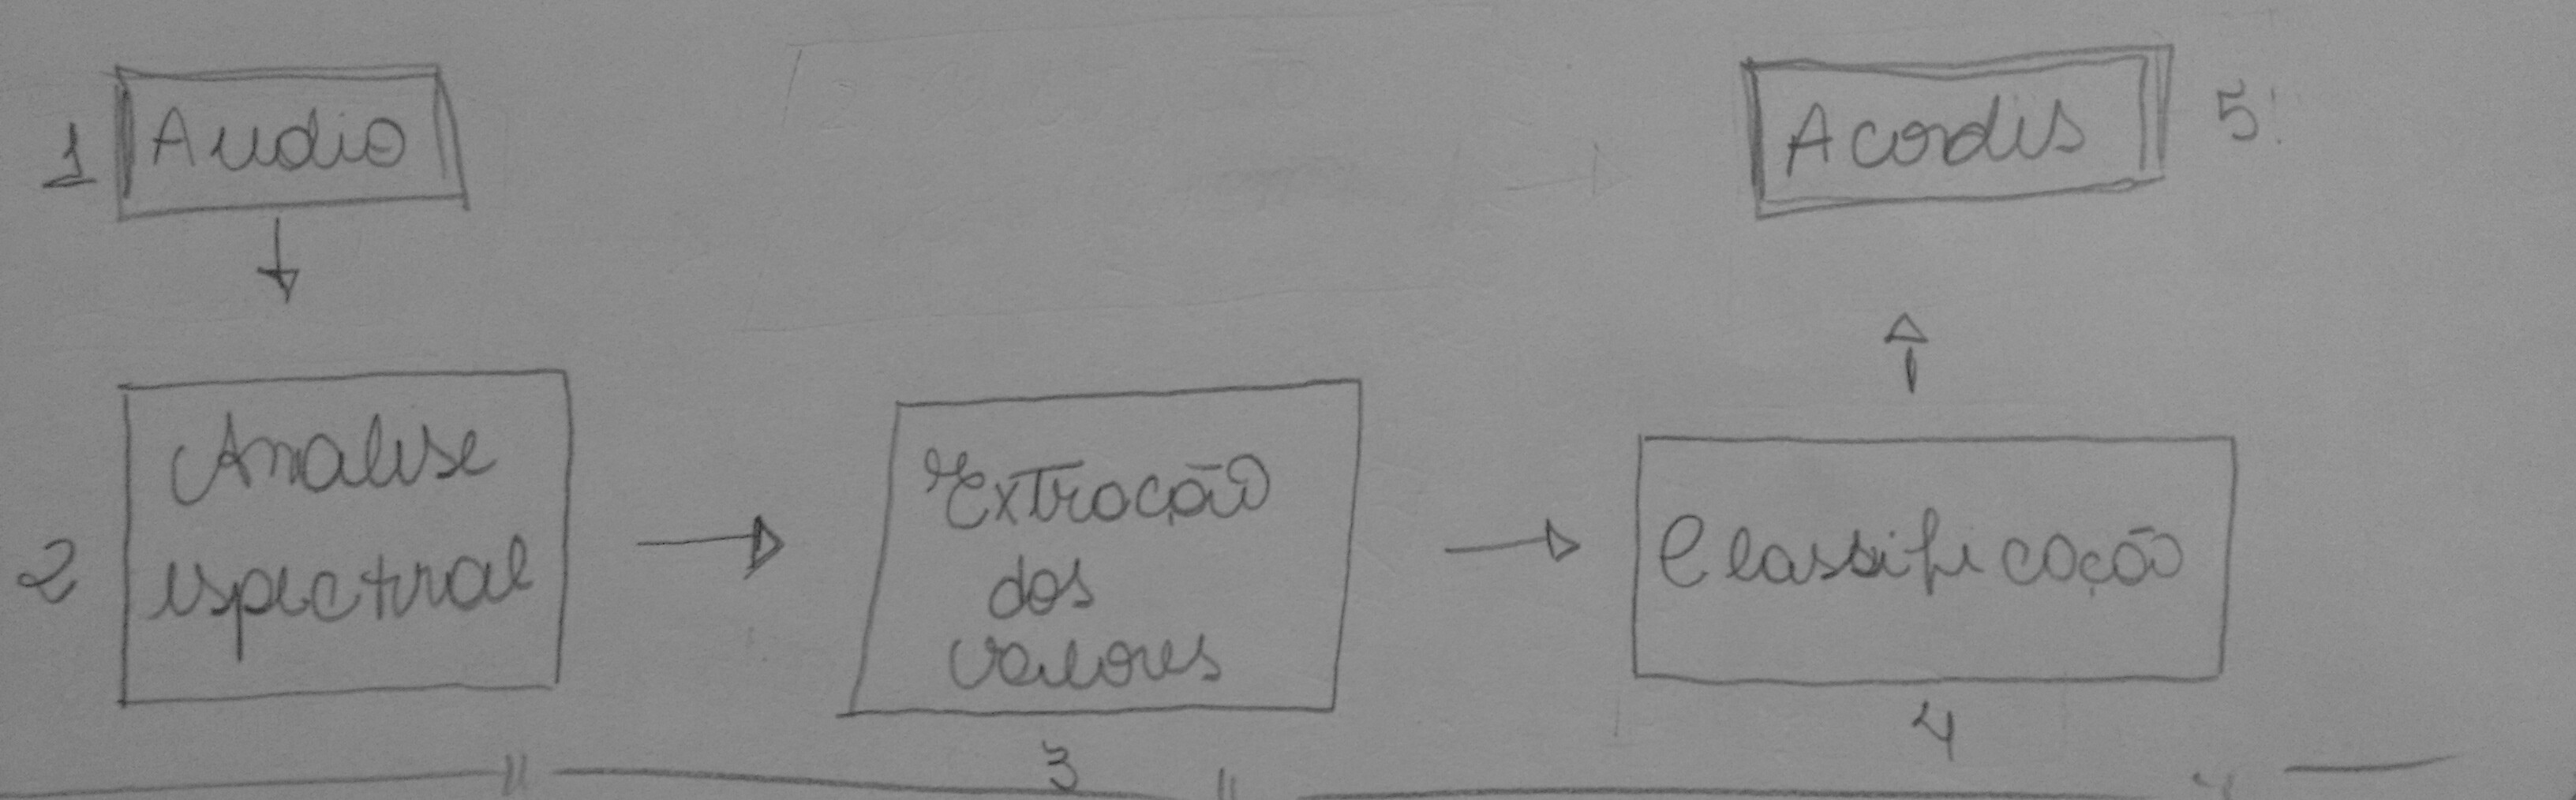
\includegraphics[scale=0.15]{figuras/IMG_20171110_144014.jpg}
     \caption{Diagrama da Metodologia}
     \label{metodologia}
\end{figure} 

% OBS: vou criar essa figura ainda

\section{Áudio}
\label{cap:audio}
Para que uma frenquência seja compreendida pelo ouvido humano, ela precisa ser repetida periodica. Por isso a entrada de áudio no formato WAVE, precisa ser fracionada e repetida perioticamente, essa quebra no audio é necessário para que se possa realizar uma analise espectral dessa frequência usando transformada rapida de Fourier.


\section{Analise Espectral}
\label{cap:analise:espectral}
Aplicamos transformada rapida de Fourier ao sinal de entrada pois precisamos trazer o audio de dominio do tempo, para o domínio da frequência, a saida dessa aplicação é o espctro de Fourier, onde conseguimos observar as notas separadamente e assim podemos armazenar esses dados nos vetores croma.


\section{Extração de Valores}
\label{cap:extraçaõ:valores}
Para construção dos vetores croma é necessário uma nota inicial F0.
Sendo F0 uma das notas temperadas da tabela de acordes. Podemos obter essa nota atraves de uma equação pré definida.
Que no caso não definimos ainda, pois não foram realizados testes nessa etapa do trabalho.

Com base no espectro de Fourier obtido através da Transformada rapida de Fourier separamos as faixas de frequência em torno da F0. 
O tamanho das faixas é um ponto importante, elas não podem ser grandes demais,pois corremos o risco de englobarem frequências intermediárias, que não nos interessam e também não podem ser muito pequenas, pois não incluiriam pequenas desafinações. Somos assim obrigados a encontrar uma solução de compromisso entre robustez e seletividade.
Para introduzirmos essa robutez desejada podemos manipular um pouco a largura dessa faixa, deixando ela um pouco mais larga que a faixa de frequencia sugerida pela F0, pois assim podemos eliminar ruidos. Sendo eles, vozes no fundo, mudanças de corda de nilon e corda de aço ou desafinação do instrumento.

Após a detecção das faixas de frequência utilizaremos da técnica de extração de picos do espectro de Fourier para construção do vetor croma, como mostra o exemplo da  \cref{extracaoPicos}.

\begin{figure}[!htb]
     \centering
     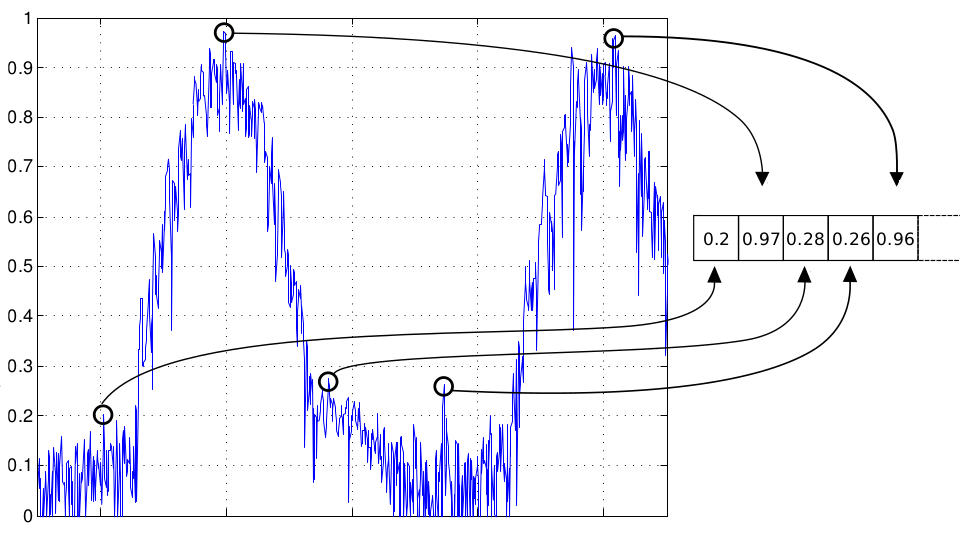
\includegraphics[scale=0.5]{figuras/picos2.png}
     \caption{Extração de picos do espectro de Fourier}
     \label{extracaoPicos}
\end{figure} 


\section{Classificador}
\label{cap:classificador}

A proposta de classificação de acordes poderá ser feita através de redes neurais artificial.
Onde usaremos uma base de dados utilizando musicas de dominio publico, com essa base de dados faremos o teste, o treinamento e a validação da rede neural artificial.

As amostras de teste e treinamento, seriam baseadas na tabela de 12 acordes e suas variações (formas diferentes de se tocar uma mesma nota) para cada acorde. 
Repetindo esses acordes para um violao com corda de aço e um violao com corda de nilon.
Podemos assim ter uma probabilidade de acerto maior para os acordes referentes ao audio de entrada.

Apos o uso dessa base de dados, podemos então aplicar essa rede neural, treinada, testada e validada nos vetores croma, para assim definirmos quais são os acordes presentes nesses vetores de croma.

Qual rede neural artificial será usado nesse trabalho ainda não foi definido, pois precisamos realizar testes para identificarmos qual rede neural teria uma porcentagem de acerto melhor para essa proposta.

\section{Acordes}
\label{cap:acrodes}
Apos aplicação das redes neurais artificias como metodo de classificação, esperamos que a saída desse sistema contenha o acorde referente ao sinal de frequência de entrada;


%---------------------------------------------------%
% \section{Considerações Finais}
% \label{cap:metodologia:sec:consideracoes:finais}

% Esta é uma sugestão de seção para dar um fechamento em cada uma dos capítulos.

% (ATENÇÃO - veja com o seu orientador se é uma seção necessária (pois trate-se de estilo de escrita)) % Esse capítulo e nome é apenas uma sugestão.
% ATENÇÃO - veja com o seu orientador se você vai ter este capítulo e se este vai ter nome!
%\chapter{Proposta}
%\label{cap:proposta}

% Esse capítulo é mais indicado para TCC 1, no qual o aluno pode expor melhor qual é a proposta de seus trabalho para a realização do TCC 1 e 2. Bem como o cronograma para realização das atividades.

% (ATENÇÃO - veja com o seu orientador se você vai ter este capítulo e se este vai ter nome!)


%---------------------------------------------------%
\chapter{Cronograma de Atividades}
\label{cap:proposta:sec:cronograma}

% (ATENÇÃO - Esta é apenas uma sugestão de elaboração de cronograma, veja com seu orientador!)

% Em TCC 1 talvez seja interessante apresentar uma cronograma de realização das atividades da proposta que englobe as atividades do TCC 2.

Nesta seção são apresentadas as atividades a serem desenvolvidas para a execução da proposta. O cronograma de realização das tarefas é apresentado na Tabela~\ref{tab:cronograma}.

\begin{enumerate}
%\item \textbf{Escrita do Projeto TCC 1.}
%\item \textbf{Estudo de Técnicas...}
%\item \textbf{Implementação da Ferramenta ...}
%\item \textbf{Testes com o conjunto de \textit{benchmarks}.}
%\item \textbf{Estudo de técnicas de Escalonamento de Tarefas.}
%\item \textbf{Entrega do TCC 1}
%\item \textbf{Apresentação do TCC 1}
%\item \textbf{Realização de Experimentos.}
\item \textbf{Estudos das ferramentnas a serem desenvolvidas para o TCC 2}
\item \textbf{Atividade do TCC 2}
\item \textbf{Implementação da metodologia proposta no TCC 1}
\item \textbf{Treinamento e teste das ferramentas desenvolvidas na metodologia}
\item \textbf{Escrita do TCC2}
\item \textbf{Entrega do TCC 2.}
\item \textbf{Apresentação do TCC 2.}
\end{enumerate}

\begin{table}[h!]
\renewcommand{\arraystretch}{1.3}
\caption{Cronograma de atividades}
\label{tab:cronograma}
\scalefont{0.9}
\begin{tabular}{|c|c|c|c|c|c|c|c|c|c|c|c|c|}
\hline
\multirow{2}{*}{\textbf{\textbf{Atividade}}} & \multicolumn{4}{c|}{\textbf{2017}}& \multicolumn{8}{c|}{\textbf{2018}} \\ \cline{2-13} 
& \multicolumn{1}{l|}{\textbf{Set}} & \multicolumn{1}{l|}{\textbf{Out}} & \multicolumn{1}{l|}{\textbf{Nov}} & \multicolumn{1}{l|}{\textbf{Dez}} & \multicolumn{1}{l|}{\textbf{Jan}} & \multicolumn{1}{l|}{\textbf{Fev}} & \multicolumn{1}{l|}{\textbf{Mar}} & \multicolumn{1}{l|}{\textbf{Abr}} & \multicolumn{1}{l|}{\textbf{Mai}} & \multicolumn{1}{l|}{\textbf{Jun}} & \multicolumn{1}{l|}{\textbf{Jul}} & \multicolumn{1}{l|}{\textbf{Ago}} \\ \hline
\textbf{1}  & X &   &   &   &   &   &   &   &   &   &   &  \\ \hline
\textbf{2}  & X & X & X & X &   &   &   &   &   &   &   &  \\ \hline
\textbf{3}  &   & X & X & X & X & X &   &   &   &   &   &  \\ \hline
\textbf{4}  &   &   & X & X & X & X &   & X & X &   &   &  \\ \hline
\textbf{5}  &   &   & X & X & X &   &   &   &   &   &   &  \\ \hline
\textbf{6}  &   &   & X & X & X & X & X & X & X & X &   &  \\ \hline
\textbf{7}  &   &   & X & X &   & X & X &   & X & X &   &  \\ \hline
\textbf{8}  &   &   &   & X & X &   & X & X &   & X & X &  \\ \hline
\textbf{9}  &   &   &   &   & X & X & X & X & X & X & X & X \\ \hline
\textbf{10} &   &   &   &   &   &   &   &   &   &   &   & X \\ \hline
\end{tabular}
\end{table}

%---------------------------------------------------%
% \section{Considerações Finais}
% \label{cap:proposta:consideracoes:finais}

% Esta é uma sugestão de seção para dar um fechamento em cada uma dos capítulos.

% (ATENÇÃO - veja com o seu orientador se é uma seção necessária (pois trate-se de estilo de escrita)) % Esse capítulo e nome é apenas uma sugestão (bom para TCC 1).
% % ATENÇÃO - veja com o seu orientador se você vai ter este capítulo e se este vai ter nome!
\chapter{Experimentos e Resultados} 
\label{cap:experimentos:resultados}

Texto de ligação/introdução do capítulo...

(ATENÇÃO - veja com o seu orientador se você vai ter este capítulo e se este vai ter nome!)

%sugestão de seção
\section{Experimentos}
\label{cap:experimentos:sec:resultados:experimentos}

Descreva os experimentos realizados...

(ATENÇÃO - Essa seção é uma sugestão, veja com o seu orientador se você vai ter essa e se vai ter esse nome!)

TEXTO TEXTO TEXTO TEXTO TEXTO TEXTO TEXTO TEXTO TEXTO TEXTO TEXTO TEXTO TEXTO TEXTO TEXTO TEXTO TEXTO TEXTO TEXTO TEXTO TEXTO TEXTO TEXTO TEXTO TEXTO TEXTO TEXTO TEXTO TEXTO TEXTO TEXTO TEXTO TEXTO TEXTO TEXTO TEXTO TEXTO TEXTO TEXTO TEXTO TEXTO TEXTO TEXTO TEXTO TEXTO TEXTO TEXTO TEXTO TEXTO TEXTO TEXTO TEXTO TEXTO TEXTO TEXTO TEXTO TEXTO TEXTO TEXTO TEXTO TEXTO TEXTO TEXTO TEXTO TEXTO TEXTO TEXTO TEXTO TEXTO TEXTO TEXTO TEXTO TEXTO TEXTO TEXTO TEXTO TEXTO TEXTO TEXTO TEXTO TEXTO TEXTO TEXTO TEXTO TEXTO TEXTO TEXTO TEXTO TEXTO TEXTO TEXTO TEXTO TEXTO TEXTO TEXTO TEXTO TEXTO TEXTO TEXTO TEXTO TEXTO TEXTO TEXTO TEXTO TEXTO TEXTO TEXTO TEXTO TEXTO TEXTO TEXTO TEXTO TEXTO TEXTO TEXTO TEXTO TEXTO TEXTO TEXTO TEXTO TEXTO TEXTO TEXTO TEXTO TEXTO TEXTO TEXTO TEXTO TEXTO TEXTO TEXTO TEXTO

%sugestão de seção
\section{Resultados}
\label{cap:experimentos:resultados:sec:resultados}

Aqui você pode descrever os resultados obtidos nos experimentos e/ou analisar/discutir tais resultados.

(ATENÇÃO - Essa seção é uma sugestão, veja com o seu orientador se você vai ter essa e se vai ter esse nome!)

TEXTO TEXTO TEXTO TEXTO TEXTO TEXTO TEXTO TEXTO TEXTO TEXTO TEXTO TEXTO TEXTO TEXTO TEXTO TEXTO TEXTO TEXTO TEXTO TEXTO TEXTO TEXTO TEXTO TEXTO TEXTO TEXTO TEXTO TEXTO TEXTO TEXTO TEXTO TEXTO TEXTO TEXTO TEXTO TEXTO TEXTO TEXTO TEXTO TEXTO TEXTO TEXTO TEXTO TEXTO TEXTO TEXTO TEXTO TEXTO TEXTO TEXTO TEXTO TEXTO TEXTO TEXTO TEXTO TEXTO TEXTO TEXTO TEXTO TEXTO TEXTO TEXTO TEXTO TEXTO TEXTO TEXTO TEXTO TEXTO TEXTO TEXTO TEXTO TEXTO TEXTO TEXTO TEXTO TEXTO TEXTO TEXTO TEXTO TEXTO TEXTO TEXTO TEXTO TEXTO TEXTO TEXTO TEXTO TEXTO TEXTO TEXTO TEXTO TEXTO TEXTO TEXTO TEXTO TEXTO TEXTO TEXTO TEXTO TEXTO TEXTO TEXTO TEXTO TEXTO TEXTO TEXTO TEXTO TEXTO TEXTO TEXTO TEXTO TEXTO TEXTO TEXTO TEXTO TEXTO TEXTO TEXTO TEXTO TEXTO TEXTO TEXTO TEXTO TEXTO TEXTO TEXTO TEXTO TEXTO TEXTO TEXTO TEXTO TEXTO

%---------------------------------------------------%
\section{Considerações Finais}
\label{cap:experimentos:resultados:sec:consideracoes:finais}

Esta é uma sugestão de seção para dar um fechamento em cada uma dos capítulos.

(ATENÇÃO - veja com o seu orientador se é uma seção necessária (pois trate-se de estilo de escrita)) % Esse capítulo e nome é apenas uma sugestão.
% \chapter{Conclusões}
\label{cap:conclusoes}

Texto de ligação/introdução da conclusão...

%sugestão de seção
\section{Considerações finais ou parciais}
\label{cap:conclusoes:sec:consideracoes:finais:parciais}

Descreva as conclusões parciais (TCC1) e finais (TCC2) do seu trabalho.

(ATENÇÃO - Essa seção é uma sugestão, veja com o seu orientador se você vai ter essa e se vai ter esse nome!)

TEXTO TEXTO TEXTO TEXTO TEXTO TEXTO TEXTO TEXTO TEXTO TEXTO TEXTO TEXTO TEXTO TEXTO TEXTO TEXTO TEXTO TEXTO TEXTO TEXTO TEXTO TEXTO TEXTO TEXTO TEXTO TEXTO TEXTO TEXTO TEXTO TEXTO TEXTO TEXTO TEXTO TEXTO TEXTO TEXTO TEXTO TEXTO TEXTO TEXTO TEXTO TEXTO TEXTO TEXTO TEXTO TEXTO TEXTO TEXTO TEXTO TEXTO TEXTO TEXTO TEXTO TEXTO TEXTO TEXTO TEXTO TEXTO TEXTO TEXTO TEXTO TEXTO TEXTO TEXTO TEXTO TEXTO TEXTO TEXTO TEXTO TEXTO TEXTO TEXTO TEXTO TEXTO TEXTO TEXTO TEXTO TEXTO TEXTO TEXTO TEXTO TEXTO TEXTO TEXTO TEXTO TEXTO TEXTO TEXTO TEXTO TEXTO TEXTO TEXTO TEXTO TEXTO TEXTO TEXTO TEXTO TEXTO TEXTO TEXTO TEXTO TEXTO TEXTO TEXTO TEXTO TEXTO TEXTO TEXTO TEXTO TEXTO TEXTO TEXTO TEXTO TEXTO TEXTO TEXTO TEXTO TEXTO TEXTO TEXTO TEXTO TEXTO TEXTO TEXTO TEXTO TEXTO TEXTO TEXTO TEXTO TEXTO TEXTO TEXTO

%sugestão de seção
\section{Sugestões para Trabalhos Futuros}
\label{cap:conclusoes:sec:trabalhos:futuros}

Descreva como é possível continuar esse trabalho, ou suas ideias depois desse trabalho.

(ATENÇÃO - Essa seção é uma sugestão, veja com o seu orientador se você vai ter essa e se vai ter esse nome!)

TEXTO TEXTO TEXTO TEXTO TEXTO TEXTO TEXTO TEXTO TEXTO TEXTO TEXTO TEXTO TEXTO TEXTO TEXTO TEXTO TEXTO TEXTO TEXTO TEXTO TEXTO TEXTO TEXTO TEXTO TEXTO TEXTO TEXTO TEXTO TEXTO TEXTO TEXTO TEXTO TEXTO TEXTO TEXTO TEXTO TEXTO TEXTO TEXTO TEXTO TEXTO TEXTO TEXTO TEXTO TEXTO TEXTO TEXTO TEXTO TEXTO TEXTO TEXTO TEXTO TEXTO TEXTO TEXTO TEXTO TEXTO TEXTO TEXTO TEXTO TEXTO TEXTO TEXTO TEXTO TEXTO TEXTO TEXTO TEXTO TEXTO TEXTO TEXTO TEXTO TEXTO TEXTO TEXTO TEXTO TEXTO TEXTO TEXTO TEXTO TEXTO TEXTO TEXTO TEXTO TEXTO TEXTO TEXTO TEXTO TEXTO TEXTO TEXTO TEXTO TEXTO TEXTO TEXTO TEXTO TEXTO TEXTO TEXTO TEXTO TEXTO TEXTO TEXTO TEXTO TEXTO TEXTO TEXTO TEXTO TEXTO TEXTO TEXTO TEXTO TEXTO TEXTO TEXTO TEXTO TEXTO TEXTO TEXTO TEXTO TEXTO TEXTO TEXTO TEXTO TEXTO TEXTO TEXTO TEXTO TEXTO TEXTO TEXTO TEXTO % Esse capítulo e nome é apenas uma sugestão.

% Apendices.
% \appendix
% \chapter{Instalação de Ferramentas}
\label{ape:instalacao:ferramentas}

Os apêndices são usados para disponibilizar materiais extras que por questões de espaço ou estilo de escrita não foram colocados diretamente no texto. Por exemplo, \textit{scripts}, instruções de instalação das ferramentas utilizadas pelo trabalho, partes de código fonte e questionários que tenham sido aplicados, tabelas com resultados...

(ATENÇÃO - veja com o seu orientador se é necessário disponibilizar algum material extra sobre algum capítulo em anexo!)



%bibliografia
\bibliographystyle{abntex2-alf}
\bibliography{main} % geração automática das referências a partir do arquivo main.bib

\backmatter
\end{document}
